% ######################################################################
%
% 			PREAMBULE
%
% ######################################################################

% -------------------------------------------------------
% Ce document est un raport. dizaine de pages / plusieurs sections
% -------------------------------------------------------
\documentclass[a4paper,12pt]{report}

% -------------------------------------------------------
% Utiliser latin1 pour les accents
% ne pas utiliser utf8 et Latex n'aime pas utf8 ET latin1
%\usepackage[utf8]{inputenc}
% -------------------------------------------------------
\usepackage[utf8]{inputenc}

% Vu dans un forum : utiliser plutôt frenchb, french est obsolete
\usepackage[T1]{fontenc}
\usepackage[english,frenchb]{babel}

% -------------------------------------------------------
% Trouvé dans un forum a voir plus tard
% utile ou pas
% significations
% -------------------------------------------------------
\usepackage{amsmath}
\usepackage{amssymb,amsfonts,textcomp}
\usepackage{color}
\usepackage{array}
\usepackage{supertabular}
\usepackage{hhline}
\usepackage{hyperref}
\usepackage{lmodern}
% \usepackage{unicode-math}	% pour prime dprime tprime

% -------------------------------------------------------
% Théorèmes
% -------------------------------------------------------
\usepackage{amsthm}
\theoremstyle{plain}				% Choix du style
\newtheorem{theoreme1}{Théorème}	% Définition de l'environnement 1

\theoremstyle{definition}				% Choix du style
\newtheorem{definition1}{Definition} %[section]	% Définition de l'environnement définition
% -------------------------------------------------------
%pour utiliser
% \textsubscript{}
% {\textbar}
% -------------------------------------------------------
\usepackage{fixltx2e}

% -------------------------------------------------------
%BIBTEX
% -------------------------------------------------------
\usepackage{natbib}

%____________________________________________________________________
%
% Tout ceci ne fonctionne pas ! ou n'ai pas réussi à faire fonctionner
% \usepackage[backend=bibtex, style=numeric]{biblatex}	% Compilateur
% \bibliography{Bibliographie}			% Utilise Bibliographie.bib
% \addbibresource{Bibliographie.bib}
% \bibliographystyle{plain}
%____________________________________________________________________

% -------------------------------------------------------
% Pour les tableaux
% -------------------------------------------------------
%\usepackage{slashbox}
\usepackage{diagbox} % barre oblique pour les cellule à 2 entrées


% -------------------------------------------------------
% Pour les ALGORITHMES
% linesnumbered	: les lignes sont numérotées
% ruled			: Le caption est en haut et bordé de lignes horizontale
% vlined		: Regroupement des bloc d'instructions par ligne verticales
% -------------------------------------------------------
\usepackage[linesnumbered, ruled, vlined]{algorithm2e}
\SetKwProg{Init}{init}{}{}
% mettre les commentaire des algos en bleu
\usepackage{xcolor}
\newcommand\commentairesBleus[1]{\footnotesize\ttfamily\textcolor{blue}{#1}}
\SetCommentSty{commentairesBleus}

% -------------------------------------------------------
% Information PDF généré
% -------------------------------------------------------
\hypersetup{pdftex, colorlinks=true, linkcolor=blue, citecolor=blue, filecolor=blue, urlcolor=blue, pdftitle=, pdfauthor=florianColas, pdfsubject=, pdfkeywords=}
\usepackage[pdftex]{graphicx}

% -------------------------------------------------------
% MACRO
% -------------------------------------------------------
% Pm||Cmax
\newcommand\problemGrahamPm{$P_m||C_{\max}$}
% P2||Cmax
\newcommand\problemGrahamPII{$P_2||C_{\max}$}	%aparemment ne supporte pas les chiffres.
% P||Cax	
\newcommand\problemGrahamP{$P||C_{\max}$}

% -------------------------------------------------------
% Ajout L. Philippe
% Utilisation des Todo inline en macro --> tdi
% -------------------------------------------------------
\usepackage{todonotes}
\newcommand{\tdi}[1]{\todo[inline]{{#1}}{}}

% -------------------------------------------------------
% Information générales
% Utilisé par \maketitle
% -------------------------------------------------------
\title{Historique des travaux autour du problème $P||C_{\max}$}
\author{florian colas}
% \date{2020-05-01}
\date{\today}


% ######################################################################
%
% 			SOUVENT UTILISES
%
% ######################################################################
% Pm||Cmax 				: \problemGrahamP
% P2||Cmax 				: P\textsubscript{2}{\textbar}{\textbar}C\textsubscript{max}
% P||Cmax 				: P{\textbar}{\textbar}C\textsubscript{max}
%
% Appostrophes 			: '
%
% en italique car latin : \textit{et al.}
%
% entourer un résultat
%	\begin{center}
%	\fbox{\begin{minipage}{\linewidth}
%	bla blabla
%	\end{minipage}}
%	\end{center}


% ######################################################################
%
% 				DOCUMENT
%
% ######################################################################

\begin{document}

% =======================================================
% Page de garde
% Utilise Information générales
% Ecrit le titre + auteur + date
% =======================================================
\maketitle

% -------------------------------------------------------
% Table des matières
%
% On renomme en Sommaire (document français)
%
% On définit la profondeur de la table des matières
% -1 partie,    0 Chapitre,
% 1 Section,    2 sous sections,  3 sous sous section
% 4 Paragraphe, 5 Sous paragraphe
%
% Les sections sont numérotées 1 2 3
% -------------------------------------------------------
\renewcommand{\thesection}{\arabic{section}}
\renewcommand{\contentsname}{Sommaire}
\setcounter{tocdepth}{4}	% avant 2pour la table des matières
\setcounter{secnumdepth}{3}	% pour les section sous et sous sous et paragraphes
\tableofcontents

% =======================================================
% 1 INTRODUCTION
% =======================================================
\section{Introduction}

texte


\section{Présentation du problème}
texte
\subsection{Parallélisme}
Le parallélisme est un type d{\textquotesingle}architecture informatique
dans lequel plusieurs processeurs exécutent ou traitent une application
ou un calcul simultanément. IL aide à effectuer de grands calculs en
divisant la charge de travail entre plusieurs processeurs, capables de communiquer et de coopérer

% -------------------------------------------------------
% FLYNN 1972
% -------------------------------------------------------
En 1972, Flynn propose une première classification des architectures parallèles \cite{5009071}. Cette taxonomie repose sur le nombre de flux de données (simple ou multiple) et le nombre de flux d'instructions (simple ou multiple).  
% -------------------------------------------------------
% TABLEAU taxonomie de Flynn
% diagbox permet d'avoir une barre oblique pour les deux entrées
% \backslashbox{Instructions}{Donnée} & Simple & Multiple NE FONCTIONNE PAS
% on cadre à gauche le tableau pour avoir plus de place
% -------------------------------------------------------
\begin{flushleft}
\begin{tabular}{|p{3.6cm}|p{6cm}|p{6cm}|}

% --------------------------
% TITRES
% --------------------------
\hline
\diagbox[width=10em]{Instructions}{Données} & Simple & Multiple \\
\hline

% --------------------------
% LIGNE SIMPLE
% --------------------------
Simple

%---------------------------
&
\textbf{SISD}

premiers PC

machine de Von Neumann


Obsolète, car tous les PC sont désormais multi-c{\oe}ur
%---------------------------
&
\textbf{SIMD}

Machines synchrones

Pipeline	%~

Exécution d'une instruction unique sur des données différentes
\\	\hline
% --------------------------
% LIGNE MULTIPLE
% --------------------------
Multiple
%---------------------------
&
\textbf{MISD}

Machines vectoriels

Tableau de processeurs

Exécute plusieurs instructions sur une même donnée
%---------------------------
&
\textbf{MIMD}

Multi processeurs à mémoire distribuée (multi-ordinateurs)

Multi processeurs à mémoire partagée (multi-c{\oe}urs)
%---------------------------
\\
\hline
\end{tabular}
Taxonomie de Flynn
\end{flushleft}
% -------------------------------------------------------
% Skilicorn 1988
% -------------------------------------------------------
En 1988, Skilicorn étoffe la taxonomie de Flynn et propose une classification plus complète \cite{86786}, basée sur l'architecture, avec 28 taxons. 
% -------------------------------------------------------
% Dasgupta 1990
% Inutile ici.
% -------------------------------------------------------
% \item en 1990, Dasqupta présente une classification, toujours orientée 
% \cite{50273}  3 si pas desactivé

% -------------------------------------------------------
% Duncan 1990
% -------------------------------------------------------
En 1990, Duncan présente une taxonomie de haut niveau \cite{44900}, reprenant les bases de la classification de Flynn, tout en incluant les architectures modernes, et celles qui n'ont pas encore été considérées comme architectures parallèle (e.g es processeurs vectoriels à chaînes de traitement).

{\centering
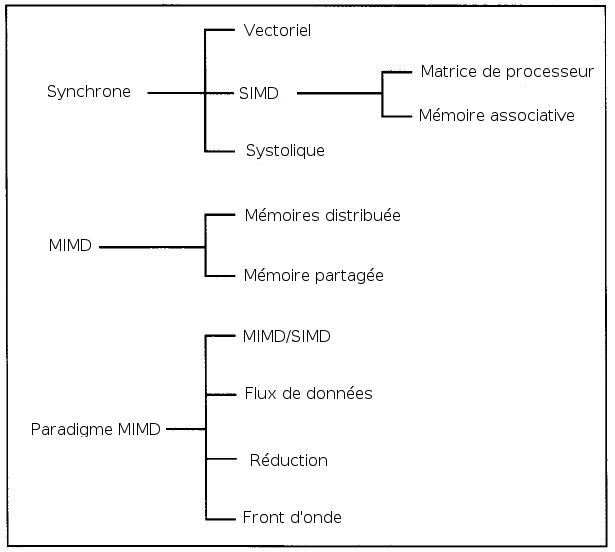
\includegraphics[width=16.272cm,height=14.605cm]{Biblio_PCmax_Rendu_Taxonomie_Duncan.jpg}
\par}
{\centering
Taxonomie de haut niveau de l'architecture de l'informatique parallèle.
\par}
 
\bigskip

\begin{itemize}
\item Les architecture synchrones. Ces architectures coordonnent les opérations concurrentes via une horloge globale et un contrôleur de programmes.(i) Les processeurs vectoriels permettent un traitement parallèle en envoyant séquentiellement des éléments vectoriels dans des pipelines d'unités de traitements mis en cascades.(ii) Les  machines systoliques, pulsent le déplacement des données entre mémoire et réseau de processeurs,à un rythme soutenu. (iii) Les SIMD, emploient une unité de contrôle centrale, et de multiples processeurs. On distingue les SIMD à matrice de processeurs, (calibrés pour le calcul scientifique à grande échelle, le traitement d'images) où on retrouve les GPU, et les SIMD à mémoire associative (particulièrement adaptés pour le traitement de bases de données, le suivi, la surveillance).
\item Les architectures asynchrones, de type MIMD, emploient plusieurs processeurs pour exécuter des flux d'instructions indépendant, en utilisant des données locales. On distingue, d'une part, les MIMD à mémoire distribuée. Les processeurs ont leur propre mémoire, et le partage d'information s'opère uniquement par échange de messages. On rencontre dans ce type d'architecture, les grappes, les MPP (Massive Parallel Processing) et les COW (Cluster Of Workstations). Et d'autre part les MIMD  à mémoire partagées, telles que les machines muti-processeurs, ou les processeurs multi-c\oe{}urs.
\item Les architectures mixtes, ou basées sur le paradigme MIMS. (i) Les hybrides MIMS/SIMS sont des architectures MIMD pilotées de la même façon que les SIMD. (ii) Les architectures à flots de données sont pilotées par les dépendances des données elles-mêmes. (iii) Les architectures à réductions sont utilisée pour les langages de programmation fonctionnels, dont les expressions sont récursives. (iv) Les architectures Front d'onde (wavefront) sont un mélange des architectures à flots de données et des architectures systoliques.





\end{itemize}



\tdi{LP: la classification de Flynn date un peu... Peut-être faut-il
  trouver qlqchose de plus récent}
\tdi{FCO: ok, fait}  



Les premières machines parallèles étaient des réseaux
d'ordinateurs, et des machines vectorielles (faiblement
parallèles, très coûteuses), telles que l'IBM 360, les
Cray1. 
\tdi{LP: Ce n'est pas si simple. On continue de faire, et d'utiliser
  des machines vectorielles, les GPU sont aussi du SIMD...}
\tdi{FCO: ok, fait}

\bigskip

{\centering
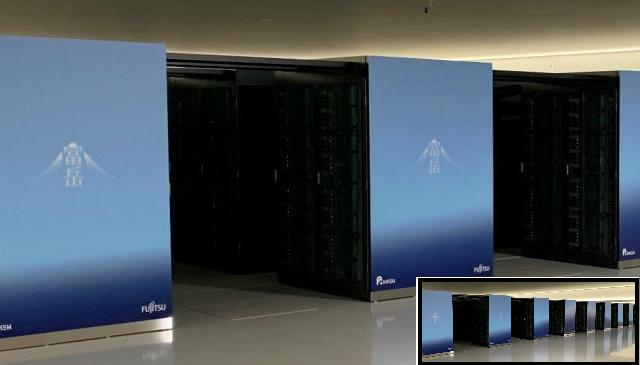
\includegraphics[width=11.29cm,height=6.44cm]{Biblio_PCmax_Rendu_Fugaku.jpg}
\par}
{\centering
Le Supercomputer Fugaku (Fujitsu), du Centre pour la science des ordinateurs de RIKEN au Japon, vient de détrôner (www.top500.org parution de juin 2020) le Summit (IBM)de l’Oak Ridge National Laboratory aux États-Unis.
Il compte 7,630,848 c\oe{}urs basés sur des processeurs ARM A64FX 48C cadencés à 2.2GHz, pour 5,087,232 GB de ram. Il fonctionne sous RedHat.
\par}

\tdi{LP: pense à compléter cette partie avec des infos sur des
  machines actuelles. voir top500.org dont il serait peut-être plus
  judicieux de citer les infos: puissance des plus gros ordinateurs,
  nombre de proc, cores, etc. Parler peut-être aussi des clouds ? Des
  applications ? Pour intro}
\tdi{FCO: ok, fait}
  
On peut définir une machine parallèle comme un ensemble de processeurs capables de coopérer et de communiquer dans le but de résoudre un problème plus rapidement. 
Les \textbf{clusters}, ou grappes (MIMD à mémoire distribuée), sont principalement homogènes. Avec internet, il devient possible d'interconnecter des ordinateurs, voire des grappes, et de créer ainsi, à l'instar d'un réseau de distribution d'électricité, un système distribué grande échelle, appelé \textbf{grid}, ou grille. Une grille relie des \textbf{ordinateurs} (PC, portable, Superordinateur, cluster), des \textbf{systèmes de bases de données} (e.g base du génome humain, atlas astronomique de Strasbourg), et dans certains cas, des \textbf{instruments spéciaux} (e.g le radio-télescope d'Arecibo). Les applications liées aux grilles sont diverses. On peut citer le web (la première grille), le \textit{"Cloud computing"}, les web-services, les réseaux \textit{"peer-to-peer"}, l'\textit{internet computing}, comme le projet SETI (www.boinc-af.org/setihome.html). Ce projet consiste à rechercher des preuves possibles de transmissions radio provenant d'intelligences, autres que terrestres, à l'aide de données fournies par un radiotélescope. Le "serveur", distribue, une portion d'échantillons radio à traiter aux clients volontaires (logiciel client installé sur un PC), pour ensuite recouper les résultats. En tout, ce sont cinq millions de participants, qui ont accumulé deux millions d'années de calculs depuis la création du projet en 1999. Se pose alors le problème de l'attribution des tâches aux clients, un problème d'ordonnancement.   


\subsection{Ordonnancement}

Sur une machine non parallèle, les tâches sont exécutées
séquentiellement, les unes après les autres.
Certaines tâches, ou jobs peuvent demander plus de temps que d'autres
pour être entièrement traitées.
Lorsque plusieurs ressources (processeurs, machines, c\oe{}urs) sont
disponibles, ou que des jobs a exécuter ne sont pas indépendants (même
traités sur un seul processeur), se pose alors, un problème
d'ordonnancement.
Celui-ci consiste à organiser, dans le temps, les jobs à exécuter, en
les affectant à une ressource donnée, de manière à satisfaire un
certain nombre de contraintes, tout en optimisant un ou des objectifs.
L'ordonnancement, fait partie de la catégorie des problèmes
d'optimisation combinatoire, et est un champ de la recherche opérationnelle, très actif depuis plus d'un siècle.

Les problèmes qui s'y rattachent sont très variés.
Premièrement, la nature des machines parallèles doit être considérée.
Celles-ci peuvent être:
\begin{itemize}
\item identiques.
  (Le même temps de traitement sera nécessaire, d'une machine à
  l'autre);
\item uniformes (un quotient de vitesse $q_i$ propre à une machine est à
  appliquer pour chaque tâche affectée à cette machine pour déterminer
  le temps de traitement nécessaire);
\item indépendantes (les temps de traitements des tâches sont ni
  uniformes ni proportionnels d'une machine à l'autre).
\end{itemize}
Ensuite, des contraintes peuvent affecter les jobs eux-mêmes.
Dans le cas d'un problème préemptif, les tâches peuvent être
interrompues, et reprises ultérieurement.
Il est possible que les jobs soient indépendants, ou au contraire,
être liées par des relations de précédence.
Ces jobs ne sont disponibles qu'à partir d'une certaine date.
Ou encore, être de durée égale, ou tous de durée différente.

Pour finir, l'objectif de
l'ordonnancement est d'optimiser un
critère. Par exemple, minimiser la somme des dates de fin, la somme
des retards, le nombre de tâches en retard, ou simplement, le retard
total. Mais le plus habituel, est de chercher à minimiser le temps
total de traitement de tous les jobs, i.e minimiser le makespan.

\tdi{LP: définir la notation de Graham à la fin de cette partie
  puisque tout y est déjà dit.}
\tdi{FCO: ok, fait}

Ces diverses possibilités définissent divers problèmes
d'ordonnancements différents, recensés et classifiés
\ par Graham et al. [1], qui introduit la notation trois-champs $\alpha
${\textbar}$\beta ${\textbar}$\gamma $ .

\bigskip

Le problème \problemGrahamP se définit alors ainsi:

\begin{itemize}

% -------------------------------------------------------
% ALPHA P Type de machines
% -------------------------------------------------------
\item $\alpha $ = $\alpha $1 $\alpha $2, détermine l'environnement
  machines.
  $\alpha $ = P: Les machines sont parallèles et identiques: Un job,
  une tâche prendra le même temps de traitement qu'il soit exécuté sur
  une machine ou une autre.
  Le nombre de machines (m) est variable.

% -------------------------------------------------------
% BETA Contraintes
% -------------------------------------------------------
\item $\beta $ $\subset$ \{ $\beta $1, $\beta $2, $\beta $3,
  $\beta $4, $\beta $5, $\beta $6\}, détermine les caractéristiques
  des jobs, ou des tâches.
  $\beta $ est vide.
  Ce qui signifie que la préemption n'est pas autorisée (les jobs
  doivent être exécutés d'une traite, sans interruption ni coupure) \
  et qu'il n'y a pas de relation entre les jobs (ils sont
  indépendants).

% -------------------------------------------------------
% GEMEL Optimisation
% -------------------------------------------------------
\item $\gamma $ détermine le critère à optimiser.
$\gamma $ = C\textsubscript{max}: on cherche à optimiser le makespan,
i.e le temps de traitement total.

\end{itemize}

\bigskip

% P{\textbar}{\textbar}C \textsubscript{max}
\subsection{Énoncé du \problemGrahamP}



\begin{definition1}{\problemGrahamP}

  \problemGrahamP consiste à planifier un ensemble $J~=~\{j_1,j_2,{\dots},j_n)$
  de n jobs simultanés, pour être traités par m machines identiques et
  parallèles.
  Chaque job, qui requière une opération, peut être traité par une des
  m machines.
  Le temps de traitement de chaque job $p_i$ (avec $i~{\in} \mathbb{N}$ ) est connu à l'avance.
  Un job commencé, et complété sans interruption.
  Les jobs, indépendants, sont exécutés par une seule machine, et une
  machine ne peut traiter qu'un seul job à la fois.

la notation :
\begin{itemize}
\item \problemGrahamP ~ou \problemGrahamPm ~précise que le nombre de machines $m$ est fixe, et est connu à l'avance dans l'instance du problème, mais reste une variable. 
\item  \problemGrahamPII fixe le nombre de machines parallèles. ici, deux.
\end{itemize}

\end{definition1}




\tdi{LP: on peut recontextualiser l'intérêt du problème. A l'heure
  actuelle, bon nombre de centres de calcul ont un parc
  assez homogène. De même les clouds offrent des instances de VM, ce
  qui permet d'avoir un environnement d'exec homogène }

\tdi{LP: faire un dessin illustratif ?}

\tdi{LP: dire que la difficulté repose uniquement sur le regourpement
  des jobs sur une machine puisque les machines sont identiques}
\todo{FCO: Rechercher exemples}
\subsection{Problématique}

Comme l'ont démontré Garey et Johnson,
\problemGrahamPII est un
problème NP-Difficile \citep{garey1978strong}, et
\problemGrahamP est un problème NP-Difficile
au sens fort \citep{garey1982computers}.
Cependant, \problemGrahamP devient un problème NP-Difficile, du moment
que le nombre de machines est fixé \cite{chen1999potts}, comme l'a
montré Rothkopf \cite{rothkopf1966scheduling}, qui a présenté un
algorithme de programmation dynamique.

Donner la solution optimale à un problème d'ordonnancement (dans notre
cas \problemGrahamP) n'est pas réaliste.
Même pour un problème de taille modeste, la résolution de celui-ci
demanderait un temps excessif et donc rédhibitoire.

La résolution du problème d'ordonnancement va reposer sur des méthodes
d'approche\todo{LP: approximation?}\todo{FCO: c'est bien le bon terme}, qui consistent à calculer en
temps polynomial, une solution ``assez'' proche de la valeur optimale.

Dans la littérature, l'étude d'ordonnancement est très riche et
abondante.
Le but étant d'améliorer le temps de calcul, et d'approcher le
résultat optimal.

\section{Résoudre le problème}

Comme évoqué précédemment, l'existence d'une solution qui résout le
problème n'est pas pensable, à moins que P = NP.

\subsection{Notations utilisées}

Chaque document utilise sa propre notation, mais les notions sont les mêmes.
Soient les données du problème

\begin{itemize}
% -------------------------------------------------------
% ENSEMBLE DES JOBS J
% -------------------------------------------------------
\item un ensemble de n jobs (ou tâches) $J = \{J_1, J_2, ..., J_n\}$ dont chaque
  job $J_j$ a un temps de traitement connu $P_j ~ \in ~ P = \{P_1, P_2, ..., P_n\}$

% -------------------------------------------------------
% ENSEMBLE DES MACHINES M
% -------------------------------------------------------
\item un ensemble de m machines parallèles identiques $M = \{M_1, M_2, \ldots, M_m\}$

  \tdi{LP: au besoin définir $M = \{ m_1, m_2, \ldots, m_m \}$ mais du
  coup il faut choiir à quoi sert le $m$}
  \tdi{FCO: M (majuscule) est l'ensemble des m machines parallèles identiques. $m_i$ est une machine de M, avec $1<= i<= m$, il y a double emploi entre m la machine et m le nombre de machines, mais m en tant que nombre est utilisé (aussi) dans \problemGrahamPm. Donc j'ai tout mis en majuscule lorsqu'il s'agit d'une entité, (machine, job, temps) et en minuscule, pour les nombres}

% -------------------------------------------------------
% RESULTAT DE L'ALGORITHME A
% -------------------------------------------------------
\item $C_m^A(J)$ Le résultat (makespan) de l'ordonnancement d'un
  ensemble J de jobs, sur m machines parallèles, identiques, obtenu
  par l'algorithme A.
  \tdi{LP: à quoi sert $j$ ici ?}
  \tdi{FCO  ok, fait : C'était une erreur de frappe ...le copier/coller qui va avec}

% -------------------------------------------------------
% RESULTAT OPTIMAL
% -------------------------------------------------------
\item $C_j^\star(J)$ Le makespan optimal, idéal, de l'ordonnancement d'un
  ensemble J de jobs, sur m machines parallèles identiques.
  \tdi{LP: idem}
\tdi{FCO: ok, fait}
% -------------------------------------------------------
% RATIO OBTENU/OPTIMAL
% -------------------------------------------------------
\item $\Gamma(A)=\dfrac{C_m^A(J)}{C_m^\star(J)}$ Le ratio d'approximation atteint par l'algorithme A au pire cas.

  \tdi{LP: idem}
  \tdi{FCO: ok, fait}
\end{itemize}

\subsection{Heuristiques}

\tdi{LP: définir heuristic ?}
\tdi{FCO: ok, fait}

Le but d'une heuristique (du grec \textit{heuriskein} : trouver) est de trouver une solution respectant les contraintes du problème, et de bonne qualité selon le critère d'optimisation considéré. La solution ne sera pas forcément optimale, mais une heuristique efficace tente de trouver une solution de bonne qualité, suivant le temps de résolution imparti. e.g pour le voyageur de commerce, on peut choisir l'heuristique "du plus proche voisin". on choisit la ville la plus proche de la ville courante, jusqu'à avoir visité toutes les villes. Cette heuristique est simple, mais donne un très mauvais résultat.
   
%Les heuristiques présentent plusieurs avantages. Leur complexité est
%réduite\tdi{LP: ça dépend de leur conception}, et obtiennent de bonne
%performances\tdi{LP: ça dépend aussi, je suis capable de faire des
%heuristiques non performantes}. 
Ces algorithmes donnent des résultats, dont la borne minimale $ max_j\{P_j\} \le C_m^A(J)_{minimal} \le \dfrac{\sum_{j=1}^{n} P_j}{m}$ \todo{FCO: Trouver référence dans les publis} et la borne maximale (au pire des cas $C_m^A(J)_{maximal}$ n'est pas maîtrise. une étude du comportement est nécessaire pour définir cette borne maximum.
 
Les heuristiques représentent la plus grande partie des recherches concernant le problème
d'ordonnancement. 

%même si leurs performances, au pire cas, ne sont pas\todo{LP: ??}\todo{FCO : pour dire %que, contrairement aux PTAS, le ratio n\ap est pas maîtrisé} garanties.
%Sont abordées ici les heuristiques les plus présentes dans la littérature.

\tdi{LP: on a aussi une borne min qui est le max entre la plus grande
  des tâches et sum(pi)/m}
\tdi{FCO: ok, fait}
  
\subsubsection{Basé LS (List Scheduling)}
% '

L'idée d'une LS est de stocker l'ensemble des jobs dans celle-ci, 
les trier dans un ordre particulier, 
avant de les affecter à une machine selon des règles définies.
Le premier job de la liste étant affecté à la première machine disponible.

\tdi{LP: un algorithme de liste affecte aussi un job, le premier de la
lsite, à la première machine prête}
\tdi{FCO: ok, fait}
%\bigskip
% -------------------------------------------------------
% LPT Rule
% -------------------------------------------------------
\paragraph{LPT rule (Graham \textit{et al.}, 1969)}

% Présentaion
% ---------------------
Graham propose \cite{graham1969bounds} \textit{\textbf{Longest Processing Time (LPT) rule}}.

\bigskip
% Algorithme
% ---------------------
\begin{algorithm}[H]
\DontPrintSemicolon
\KwData{instance de \problemGrahamP, avec m machines, n jobs et leur temps d'exécution}
%\Begin{ %inutile ici et rajoute un nuero de ligne

\BlankLine % Petit espace
Trie les jobs de l'ensemble J dans l'ordre décroissant de leur temps
d'exécution et ré-indexe l'ensemble de telle manière à obtenir:
$P_1 \geq P_2 \geq \ldots \geq P_n$

\BlankLine % Petit espace
Parcours la liste, et affecte chaque job à la machine la moins
chargée, à ce moment là.
% }
\caption{LPT Rule\label{LPT}}
\end{algorithm}
\todo{FCO: Algo en anglais}
\bigskip
% Exemple
% ---------------------
Exemple

Soit $P=\{13,10,7,6,6,5,3,2\}$, l'ensemble des $P_j$ déjà triés dans
l'ordre décroissant à appliquer sur 4 machines parallèles identiques:

{\centering
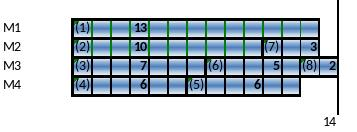
\includegraphics[width=8.334cm,height=4.034cm]{Biblio_PCmax_Rendu_exLPT1.jpg}
\par}
{\centering
\par}
Nous obtenons $C_4^{lpt}(J)=14$

\bigskip

% Complexité
% -------------------------------------------------------
\begin{flushleft}
\begin{tabular}{|p{8cm}p{6cm}|}
% TITRES (pas de titre)
\hline

% Ligne blanche
 & \\

% Ligne Complexité
Le tri puis l'affectation s'effectuent en & $O(n \log n + n \log m)$
\\	% pas de ligne \hline

% RATIO
Le ratio d'approximation	&	$\Gamma(LPT)\leq \dfrac{4}{3} - \dfrac{1}{3m}$
\\

% Ligne blanche
& \\
\hline
\end{tabular}
%pas de legende
\end{flushleft}

%\bigskip
% -------------------------------------------------------
% LPT-REV
% -------------------------------------------------------

\paragraph{LPT-REV (Croce \textit{et al.}, 2018)}

% Présentaion
% ---------------------
Le ratio d'approximation obtenu par LPT (\ref{LPT})
$(\Gamma(LPT)\leq \dfrac{4}{3} - \dfrac{1}{3m})$ est une borne
supérieure que cet algorithme peut atteindre, mais qu'il ne dépassera
jamais.
Chaque utilisation de LPT produira un résultat dont le ratio $\Gamma$
oscillera entre 1 et $\dfrac{4}{3} - \dfrac{1}{3m})$.

\bigskip
% Exemple pour l'explication
% ---------------------
Exemple de pire cas

Soit $P=\{7,7,6,6,5,5,4,4,4\}$, l'ensemble des $P_j$ déjà triés dans
l'ordre décroissant à appliquer sur 4 machines parallèles identiques:

\bigskip

% partie insécable
\begin{minipage}{\linewidth}

\begin{flushleft}
LPT donne le résultat suivant
\end{flushleft}
{\centering
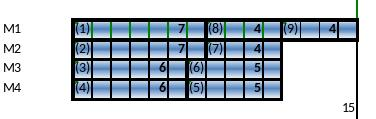
\includegraphics[width=8.334cm,height=4.034cm]{Biblio_PCmax_Rendu_exLPT_Rev1.jpg}
\par}

\begin{flushleft}
$C_4^{lpt}(J)=15$
\end{flushleft}

\end{minipage}

\bigskip

% partie insécable
\begin{minipage}{\linewidth}

\begin{flushleft}
Un ordonnancement optimal aurait été:
\end{flushleft}

{\centering
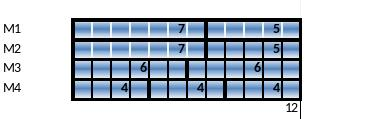
\includegraphics[width=8.334cm,height=4.034cm]{Biblio_PCmax_Rendu_exLPT_Rev2.jpg}
\par}


\begin{flushleft}
$C_4^{\star}(J)=12$
\end{flushleft}

\end{minipage}

Soit une marge de $\dfrac{15}{12}$

Le ratio d' approximation prévu pour $m=4$

$\dfrac{4}{3} - \dfrac{1}{3m}=\dfrac{16}{12} - \dfrac{1}{12}=\dfrac{15}{12}$

Ce cas, représente donc un pire cas pour LPT.

\bigskip
\begin{definition1}{Job et machine critique}

Le job critique (noté $J^\prime$) est le job qui détermine le
makespan.

La machine critique est la machine qui exécute le job critique.
\end{definition1}


\bigskip

Croce \textit{et al.}
\cite{della2018longest}, en examinant le comportement de LPT rule,
notamment au niveau du ratio d'approximation, constatent qu'icelui
peut être réduit selon certaines configurations, ou instances du
problème, et rédigent le théorème suivant:

\bigskip

\begin{theoreme1}

  LPT a un rapport d'approximation non supérieur à
  $\dfrac{4}{3} - \dfrac{1}{3(m-1)}$ pour $m \geq 3$ et $n \neq 2m+1$.

  LPT atteint la limite de Graham $\dfrac{4}{3} - \dfrac{1}{3m}$ pour
  $m \geq 2$ et uniquement dans le cas où $n=2m+1$, et la machine
  critique traite 3 jobs, tandis que les autres en traitent 2.

\end{theoreme1}

\bigskip

Le rapport d' $\dfrac{4}{3} - \dfrac{1}{3(m-1)}$ est inférieur au
ratio $\dfrac{4}{3} - \dfrac{1}{3m}$ (quel que soit le nombre de
machines)

\bigskip

\textbf{NB}

L'exemple précédant (pire cas) a les caractéristiques suivantes:
\begin{itemize}
	\item nombre de job $n=2m+1$.
	\item la machine critique exécute 3 jobs.
	\item les autres exécutent 2 jobs.
	\item un rapport d'approximation de $\dfrac{4}{3} - \dfrac{1}{3m}$
\end{itemize}

\bigskip

Une modification à l'algorithme LPT rule est apportée afin de placer
le problème \problemGrahamP toujours dans une instance où le ratio
d'approximation est $\leq \dfrac{4}{3} - \dfrac{1}{3(m-1)}$.
Cette modification consiste à planifier en premier, le job critique
sur une machine M1.

\bigskip
\todo{FCO: Algo en anglais}

% Algorithme
% ---------------------
\begin{algorithm}[H]
\DontPrintSemicolon
\KwData{instance de \problemGrahamP, avec m machines, n jobs}
%\Begin{ %inutile ici et rajoute un nuero de ligne

Apply LPT yielding a schedule with makespan $z_1$ and $k-1$ jobs on
the critical macine before job $J^\prime$ \BlankLine % Petit espace
Apply $LPT^\prime = LPT(J^\prime)$ with solution value $z_2$

\BlankLine % Petit espace
\textbf{If} $m=2$ \textbf{then} apply
$LPT''=LPT([(J^\prime - k + 1), ...
, J^\prime])$ with solution value $z_3$ and \textbf{return}
$min[z_1,z_2,z_3]$

\BlankLine % Petit espace
\textbf{Else} \textbf{return} $min(z_1,z_2)$

\caption{LPT-Rev\label{LPTRev}}
\end{algorithm}


\bigskip

% Complexité
% -------------------------------------------------------
\begin{flushleft}
\begin{tabular}{|p{8cm}p{6cm}|}
% TITRES (pas de titre)
\hline

% Ligne blanche
 & \\


% RATIO
Ratio d'approximation	&	$\Gamma(LPT-REV)\leq \dfrac{4}{3} - \dfrac{1}{3(m-1)}$
\\

% Ligne blanche
& \\
\hline
\end{tabular}
%pas de legende
\end{flushleft}


\subsubsection{Basé Bin-Packing}

Le problème Bin-packing, est semblable au problème \problemGrahamP.
Il consiste à ranger des objets de taille différentes, dans des bacs
identiques, tout en minimisant leur nombre.

L'ensemble des n jobs $J = \{J_1, J_2, \ldots, J_n\}$, et de leurs temps de
traitement $P_j ~ \in ~ P = \{P_1, P_2, ..., P_n\}$, peuvent être vus
respectivement comme:
\begin{itemize}
\item un ensemble d'objets $T_j ~ \in ~ T = \{T_1, T_2, ..., T_n\}$
\item leur taille $L(T_j)~ avec ~ 1 \le j \le n$
\end{itemize}
Une taille maximale $C$ des bacs (ou boites) est donnée.
\bigskip

\begin{definition1}{Packing}

  Un packing, est une partition $P<P_1, P_2, ..., P_m>$ tel que
  $L(P_i) \leq C$ avec $1 \leq i\leq m$.
  Le but est de placer les objets $T_j$ dans des bacs $P_i$ de taille
  $C$, de manière à minimiser le nombre de bacs $m$.
\end{definition1}

le problème Bin-packing est NP-Complet \cite{Johnson1974WorstCasePB}. 

L'idée est d'utiliser le problème Bin-Packing à l'envers, pour
approcher une solution au problème d'ordonnancement.

\tdi{LP: petite remarque sur la complexité du problème ?}
\tdi{FCO: ok, fait}




% -------------------------------------------------------
% MULTIFIT
% -------------------------------------------------------
\paragraph{MULTIFIT}

% Présentaion
% ---------------------
Coffman \textit{et al.}, \cite{coffman1978application} se sont
intéressés à l'algorithme FFD (First Fit Decreasing), un outil de
résolution du problème de Bin-Packing, pour l'adapter au problème
\problemGrahamP.
$FFD(T,C)$ renvoie le nombre de bacs de taille C non vides
nécessaires, et l'arrangement correspondant de l'ensemble T d'objets.

\bigskip
% Principe de l'algorithme
% ---------------------
Soit $T_m^\star = min\{C:FFD(T,C) \leq m\}$ la plus petite valeur de
$C$ (taille des bacs) qui permet à $T$ d'être pacqué dans m (ou moins)
bacs.

\bigskip

L'idée de MULTIFIT est donc de proposer une valeur pour $C$, 
faire tourner $FFD(T,C) $, 
et réduire à chaque itération cette valeur de $C$ jusqu'à ce que le nombre $m$ de bacs renvoyé par $FFD(T,C) $, alors devenu insuffisant, augmente à $m+1$.
Cette valeur charnière de $C$ est $T_m^\star$, qui correspond au
makespan minimum recherché, de l'ordonnancement de l'ensemble $T$ de
jobs sur $m$ machines identiques parallèles.
La difficulté, est de proposer une première valeur de $C$ pas trop éloignée de la valeur recherchée, afin de réduire au maximum le nombre d'itérations. 
\tdi{LP: deux mots pour dire comment est implémentée la recherche}
\tdi{FCO: ok, fait}

La méthode utilisée est une recherche dichotomique. 
Après avoir défini les bornes 
supérieure $C_u = \max\{\dfrac{2}{m} \cdot L(T), \max_i\{L(T_i)\} \}$ et 
inférieure $C_l = \max\{\dfrac{2}{m} \cdot L(T), \max_i\{L(T_i)\} \}$ de départ, 
FFD est exécuté avec le milieu $C_d = \frac{C_u + C_l}{2}$. 
si $FFD(T,C_d)\le m$ alors la nouvelle fourchette de recherche devient $C_u = C_d$ et $C_l$, 
sinon (si $FFD(T,C_d)> m$) alors la nouvelle fourchette devient  $C_u$ et $C_l = C_d$. 
Un nombre d'itérations $k$ et donné à l'exécution de MULTIFIT, estimé en fonction de la taille du problème (n et m). Mais même pour un problèmes de grande taille, le résultat ne change plus après $7$ itérations. Il est donc inutile d'utiliser $k>7$.     
  

{\centering
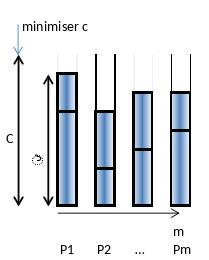
\includegraphics[width=6.138cm,height=7.62cm]{Biblio_PCmax_Rendu_exMULTIFIT1.jpg}
%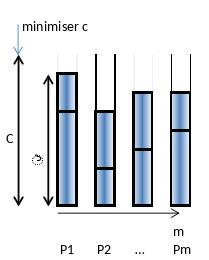
\includegraphics[width=8.334cm,height=4.034cm]{Biblio_PCmax_Rendu_exMULTIFIT1.jpg}

\par}
{\centering
Fonctionnement de FFD et principe de MULTIFIT
\par}

\bigskip
\todo{FCO: algo en anglais + enlever les goto}
% Algorithme
% ---------------------
\begin{algorithm}[H]
\DontPrintSemicolon
\KwData{T un ensemble de jobs

m, un nombre de processeurs

borne supérieure: $Cu[T,m] = \max\{\dfrac{2}{m} \cdot L(T), \max_i\{L(T_i)\} \}$

borne inférieure: $Cl[T,m] = \max\{\dfrac{1}{m} \cdot L(T), \max_i\{L(T_i)\} \}$

k un nombre d'itérations
}

\BlankLine % Petit espace
La recherche de $T_m^\star$ s'effectue par dichotomie sur k itérations

\BlankLine % Petit espace
Après les k itérations, MULTIFIT \textbf{ renvoie $Cu(k)$} qui
correspond à la plus petite valeur de $C$ pour laquelle $FFD[T,C] \leq
m$

\caption{MULTIFIT\label{MULTIFIT}}
\end{algorithm}
\tdi{LP: $k$ fixé ? ou seuil entre deux iter ?}
\tdi{FCO: ok, fait}

\bigskip

% Complexité
% -------------------------------------------------------
\begin{flushleft}
\begin{tabular}{|p{8cm}p{6cm}|}
% TITRES (pas de titre)
\hline

% Ligne blanche
 & \\

% Ligne Complexité
Tri puis k FFD s'effectuent en & $O(n \log n + kn \log m)$
\\	% pas de ligne \hline

% Ligne blanche
 & \\

% RATIO
Ratio \cite{lee1988multiprocessor} & $\Gamma(MULTIFIT) \leq 1,220 + 2^{-k}$

\\

% Ligne blanche
& \\
\hline
\end{tabular}
%pas de legende
\end{flushleft}

Généralement, MULTIFIT donne des résultats très satisfaisant avec $k = 7$


% -------------------------------------------------------
% COMBINE
% -------------------------------------------------------
\paragraph{COMBINE}

% Présentaion
% ---------------------
Lee \textit{et al.}, \cite{lee1988multiprocessor} ont l'idée
d'utiliser LPT (\ref{LPT}) pour réduire les bornes de départ 
et ainsi optimiser MULTIFIT (\ref{MULTIFIT}) dans un algorithme nommé COMBINE.

\tdi{LP: développer/préciser un peu}
\tdi{FCO: ok, fait}
\bigskip
soient
\begin{align*}
&la~moyenne~des~poids~des~jobs~par~processeur &A &= \sum_{i=1}^{n}(\dfrac{P_i}{m})\\
&et &M &= C_m^{lpt}(J) \\
& &M^\star &= C_m^\star(J)
\end{align*}

COMBINE, améliore certains point de l'algorithme MULTIFIT en se basant sur les principes suivants :
\begin{itemize}
\item Le résultat $M$ obtenu par LPT, est forcément supérieur ou égal à $M^\star$, soit $M>M^\star$. COMBINE utilise donc $M = C_m^{lpt}(J)$ comme borne supérieur $C_u$ de départ pour la recherche dichotomique utilisée par MULTIFIT. celle-ci est beaucoup plus proche du résultat optimal que la borne supérieure de départ $2\cdot A$ utilisé à l'origine par MULTIFIT.
\item Si Le résultat $M$ obtenu par LPT est tel que $M \geq 1,5\cdot A$ alors $M=M^\star$. Il n'est donc pas nécessaire de poursuivre la recherche.
\item Au lieu de prédéterminer un nombre d'itérations, COMBINE utilise une condition d'arrêt de la recherche dichotomique, en fonction de l'écart entre les deux bornes. COMBINE stope la recherche dès que $C_u - C_l \le \alpha \cdot A$. Les tests de COMBINE ont été effetués avec $\alpha = 0,005$  
\end{itemize}
 

\bigskip
\todo{FCO: Algo en anglais}
% Algorithme
% ---------------------
\begin{algorithm}[H]
\DontPrintSemicolon
\KwData{instance de \problemGrahamP, avec m machines, n jobs, et un coefficient $\alpha (0,005)$ }

A = $\sum_{i=1}^{n}(\dfrac{P_i}{m})$

\BlankLine % Petit espace

M $\leftarrow C_m^{lpt}(J)$

\BlankLine % Petit espace

\If {$M \geq 1,5 \cdot A$}
 {
 	$M^\star = M$ \;
 }
\Else
 {
	$C_u \leftarrow M$					\;
	$C_l \leftarrow \max \{(\dfrac{M}{\dfrac{4}{3}-\dfrac{1}{3 \cdot m}}),P1,1 \}$	\;
	\While {$C_u - C_l > \alpha \cdot A$}
	 {
	 appliquer MULTIFIT \;

	 } \tcp{on arrête lorsque $C_u - C_l \leq \alpha \cdot A$}
 }

\caption{COMBINE\label{COMBINE}}

\end{algorithm}


\bigskip

% Complexité
% -------------------------------------------------------
\begin{flushleft}
\begin{tabular}{|p{8cm}p{6cm}|}
% TITRES (pas de titre)
\hline

% Ligne blanche
 & \\

% Ligne Complexité
Conplexité & $O(n \log n + kn \log m)$
\\	% pas de ligne \hline

% Ligne blanche
 & \\

% RATIO
Ratio \cite{gupta2001listfit} & $\Gamma(COMBINE) \leq \dfrac{13}{12} + 2^{-k}$

\\

% Ligne blanche
& \\
\hline
\end{tabular}
%pas de legende
\end{flushleft}

avec k le nombre d'itérations pour la recherche dichotomique.
Concernant la complexité, pour atteindre
$C_u - C_l \leq \alpha \cdot A$, généralement, 6 itérations suffisent
($k=6$).
Mais COMBINE a déjà exécuté une fois LPT (k=7).




% -------------------------------------------------------
% LISTFIT
% -------------------------------------------------------
\paragraph{LISTFIT}

% Présentaion
% ---------------------
Gupta \textit{et al.}, \cite{gupta2001listfit}, ont aussi l'idée
d'utiliser MULTIFIT (\ref{MULTIFIT}), afin de réaliser l'olgorithme
LISTFIT.

Celui-ci sépare la liste des travaux en 2 sous-listes, traitée soit
dans un ordre LPT (Longest Time Processing), soit dans un ordre SPT
(Shortest Time Processing).
Puis LISTFIT combine ces 2 sous-listes en appliquant MULTIFIT à chaque
itération.

\bigskip
\todo{FCO: enlever les goto}
% Algorithme
% ---------------------
\begin{algorithm}[H]
\DontPrintSemicolon
\KwData{n, m, $p_i$ for $i=1, \ldots, n$}

%STEP 1
let $r=1$, $q=1$, and $C_{\max}=C_{\max}(LPT)$, the makespan obtained
by the LPT algorithm.
\textbf{Goto step 2}.

%STEP 2
\BlankLine % Petit espace
let $\Phi = \varnothing$, A = $\{1,...,n\}$, and $B = \varnothing$.
let $\omega_r$ be the sequence of jobs in job-list A sorted according
to ordering $\tau$.
\textbf{Goto step 3}.

%STEP 3
\BlankLine % Petit espace
let $\alpha=C_{\max}(MULTIFIT)$ be the makespan obtained by using
algorithm MULTIFIT, with $\sigma = \Phi_q \cdot \omega_r$ in step 1 of
algorithm MULTIFIT.
If $C_{\max}>\alpha$ then set $C_{\max} = \alpha$ and
$\gamma_h = \pi_h$ for $h=1,2,...,m$.
If $A \neq \varnothing$ then \textbf{goto step 4}; otherwise
\textbf{goto step 5}.

%STEP 4
\BlankLine % Petit espace
remove the last job of $\omega_r$ and place it into $B$.
Update $A$, $\Phi_q$ and $\omega_r$.
Let $\sigma = \Phi_q \cdot \omega_r$.
\textbf{goto step 3}.

%STEP 5
\BlankLine % Petit espace
If {$\tau < 2$} then set $\tau = \tau + 1$ and \textbf{goto step 2};
otherwise \textbf{goto step 6}

%STEP 6
\BlankLine % Petit espace
If $q<2$ then set $q=q+1$, $\tau = 1$, and \textbf{goto step 2};
oterwise \textbf{stop}; \tcp{The schedule where jobs in $\gamma_h$ are
  proceded on machine $h$ is an approximate solution of the
  \problemGrahamP problem with makespan
  $C_{\max}$.}

\caption{LISTFIT\label{LISTFIT}}
\end{algorithm}

\bigskip
% Complexité
% -------------------------------------------------------
\begin{flushleft}
\begin{tabular}{|p{8cm}p{6cm}|}
% TITRES (pas de titre)
\hline

% Ligne blanche
 & \\

% Ligne Complexité
Conplexité & $O(n^2 \log(n) + k \cdot n^2 \log(m))$
\\	% pas de ligne \hline

% Ligne blanche
 & \\

% RATIO
Ratio \cite{gupta2001listfit} & $\Gamma(LISTFIT) \leq \dfrac{13}{12} + 2^{-k}$

\\

% Ligne blanche
& \\
\hline
\end{tabular}
%pas de legende
\end{flushleft}

avec k le nombre d'itérations pour la recherche dichotomique.


\subsubsection{Approche gloutonne}

% -------------------------------------------------------
% SLACK
% -------------------------------------------------------
\paragraph{SLACK (Croce \textit{et al.}, 2018)}.

% Présentaion
% ---------------------
Croce \textit{et al.} \cite{della2018longest}, en effectuant la preuve
d'une borne d'approximation pour le
développement de LPT-Rev (\ref{LPTRev}), ont mis en évidence
l'importance des différences de temps entre les jobs,
ainsi que le regroupement de ceux-ci en sous-ensembles.

\tdi{LP: est-ce qu'on sait dire pourquoi ? faire une petite analyse}

notamment pour l'instance suivante:
% * pour ne pas numéroter. Juste besoin d'aligner
\begin{align*}
& Nombre~ de~ jobs &n &=2 \cdot m + 1			\\
& Avec &P_{2 \cdot m + 1} &\geq P_1 - P_m
\end{align*}
Où ils ont planifié d'abord, le job $2 \cdot m + 1$, puis un
sous-ensemble de jobs triés $\{1,...,m\}$ et pour finir un
sous-ensemble de jobs triés $\{m+1,...,2 \cdot m \}$

En résulte l'algorithme suivant:

\bigskip
% Algorithme
% ---------------------
\begin{algorithm}[H]
\DontPrintSemicolon
% \KwData{une instance ...}

%Etape 1
trier la liste des jobs dans l'ordre décroissant des temps nécessaires de traitements

%ETAPE 2
\BlankLine % Petit espace
réindexer les jobs, de manière à obtenir $P_1 \geq P_2 \geq ... \geq P_n$

%ETAPE 3
\BlankLine % Petit espace
Découper l'ensemble obtenu en $\dfrac{n}{m}$ tuples de $m$ jobs (ajout
de jobs "dummy" de taille nulle pour le dernier tuple, si $n$ n'est
pas un multiple de $m$)

%ETAPE 4
\BlankLine % Petit espace
considérer chaque tuple avec la différence de temps (SLACK) entre le
premier job du tuple et le dernier.
\begin{align*}
\{ &\{1, ..., m\} &\{m+1,..., 2 \cdot m\} &... \} \\
   &P_1 - P_m     &P_{m+1}-P_{2 \cdot m}  &...
\end{align*}


%STEP 5
\BlankLine % Petit espace
trier les tuples par ordre décroissant de "Slack" et ainsi former un nouvel ensemble
\tcp{e.g: $\{ \{m+1,..., 2 \cdot m\} \{1, ..., m\}\}$ si $P_{m+1} - P_{2 \cdot m} > P_1 - P_m$.}

%STEP 6
\BlankLine % Petit espace
applique l'ordonnancement (Affectation à la machine la moins chargée à ce moment là) à l'ensemble ainsi obtenu.

\caption{SLACK\label{SLACK}}
\end{algorithm}

\subsection{Programmation linéaire}

L'ordonnancement, et plus particulièrement \problemGrahamP s'inscrit
parfaitement dans l'énoncé d'un problème de programmation linéaire.
En effet, la fonction objectif i.e minimiser le makespan, ainsi que
les contraintes sont des fonctions linéaires.
Toutefois, les variables, et le résultat attendu sont discrets, ce qui
rend la résolution du problème nettement plus difficile comparé à une
programmation linéaire à variables continues.
Ces algorithmes, donnent une solution faisable exacte.

\paragraph{PA (Mokotoff)}

Mokotoff \cite{mokoto1999scheduling} présente un algorithme basé sur
la formulation de la programmation linéaire, en utilisant des
variables booléennes d'affectation des jobs à une machine.

\tdi{LP: définir $x_{ij}$}
% Présentaion
% ---------------------
\bigskip
La minimisation du makespan peut être posée ainsi:

Minimiser y tel que:

\begin{itemize}
\item $\sum_{j=1}^{m}x_{ij}=1$ \quad pour $1 \leq i \leq n$ 		\\
Sur toutes les machines, au moins un et un seul $x_i$ est égal à 1.	\\
Un job est affecté à une, et une seule machine.

\item $y-\sum_{i=1}^{n}P_i \cdot x_{ij} \geq 0$ \quad pour $1 \leq j \leq m$ \\
Pour une machine donnée, la somme des temps est $\leq$ à $y$.
\end{itemize}

\bigskip
Où	\quad	la valeur optimale de $y$ est $C_{\max}$

et	\quad	$x_{ij} =$

\begin{itemize}
\item 1 si le job $i$ est affecté à la machine $j$.
\item 0 si le job $i$ n'est pas affecté à la machine $j$.
\end{itemize}

 \bigskip
 Le programme linéaire est donc composé de
 \begin{itemize}
 \item $n \cdot m + 1$ variables (les variables $x_{ij}$ et la variable $y$)
 \item $n+m$ contraintes
 \end{itemize}

\bigskip
La zone F peut être définie ainsi: \\
$F=\{ (x,y) : x \in B^{n \cdot m}, y \in \mathbb{R_+} : \sum_{j=1}^{m} x_{ij}=1 ~ \forall i;
y-\sum_{i=1}^{n} P_i \cdot x_{ij} \geq 0 \forall j \}$

avec $B=\begin{bmatrix}
x_{11}&x_{\dots 1}&x_{n1}\\
x_{1 \dots}& \rotatebox{-30}{\dots}&x_{n \dots}\\
x_{1m}&x_{\dots m}&x_{nm1}
\end{bmatrix}$

\bigskip
le polytope $P$, relatif à $F$ est défini ainsi: \\
$F=\{ (x,y) : x \in \mathbb{R_+}^{n \cdot m}, y \in \mathbb{R_+} : \sum_{j=1}^{m} x_{ij}=1 \forall i;
y-\sum_{i=1}^{n} P_i \cdot x_{ij} \geq 0 \forall j	\}$

\bigskip
il est possible de construire un ensemble fini d'\textbf{inégalités} \\
$Ax+Dy \leq \overline{b}$ telles que \\
$min \{y : (x,y) \in F \} = min \{y : x \in \mathbb{R_+}^{n \cdot m}, y \in \mathbb{R_+} Ax+Dy \leq \underline{b}$ \\
% \ensuremath{^\circ} pour le symbole °
NB: Une solution $(x \ensuremath{^\circ} , y\ensuremath{^\circ}) \in P$ doit être exclue (car n'est pas un vecteur entier) si $(x\ensuremath{^\circ}, y\ensuremath{^\circ}) \notin P $

\bigskip
Des \textbf{inégalités transitoires} peuvent être générées (nombre maxi de jobs par machine) \\
$\sum_{i \in S_j} x_{ij} \leq L_j$ \quad $(L_j = h-1 \iff S_{J_h} > LB et S_{J_{(h-1)}} \leq LB)$\\
LB: Borne inférieure.

\bigskip

Pour un problème \problemGrahamP, même de taille modeste, le nombre de
variables et contrites est très important, dont certaines sont
inutiles.
L'algorithme va donc utiliser la méthode des plans sécants (Cutting
Plane Method).
\`A chaque itération , des inégalités valides sont générées, puis une
relaxation est exécutée, jusqu'à l'obtention d'une solution faisable.

\bigskip
% Algorithme
% ---------------------
\begin{algorithm}[H]
\DontPrintSemicolon

Détermination de la borne inférieure $(LB)$ suivant l'algorithme de
McNaughton \cite{mcnaughton1959scheduling}.

\BlankLine % Petit espace
Détermination de la borne Supérieure ($UB$ juste pour la nommer)
suivant l'heuristique LPT (\ref{LPT}).

\BlankLine % Petit espace
Si $LB$ coïncide avec $UB$ la solution optimale est trouvée Sinon le
processus itératif démarre.

\BlankLine
À chaque itération un programme de relaxation linéaire est résolu.dans
lequel $C_{\max}$ doit être égal à la borne inférieure actuelle
($LB$).
Si la solution obtenue est entière (donc faisable), l'algorithme
s'arrête et la solution actuelle est optimale.

\BlankLine
Sinon, des nouvelles inégalité (inégalités et/ou inégalités
transitoires) sont ajoutées à la nouvelle relaxation linéaire.Le
nouveau programme linéaire est résolu et l'algorithme s'arrête si la
solution est entière.

\BlankLine
Si la relaxation n'est pas possible, la limite inférieure ($LB$) est
augmentée d'une unité et le processus itératif redémarre.

\BlankLine
Par contre, si les inégalités ne peuvent pas être générées, un
algorithme \textit{Branch\&Bound} prend le relais pour résoudre le
problème.

\caption{PA\label{PA}}
\end{algorithm}


\subsection{Approximation}

Une catégorie d'algorithmes fournit une garantie d'approche.
Notamment les PTAS (Schéma d'Approximation en Temps Polynomial).

\paragraph{PTAS}

Un PTAS est un algorithme qui calcule, pour tout $\epsilon > 0$ donné,
une solution proche à un facteur $(1+\epsilon)$ pour un problème de
minimisation, ou $(1-\epsilon$ pour un problème de maximisation, de
l'optimal, en temps polynomial dépendant de $\epsilon$.

\bigskip
Hochbaum \textit{et al.} \cite{hochbaum1987using} proposent le premier PTAS.




\subsection{Autres approches}

\section{Synthèse}

\section{Conclusion}









\medskip


\bibliographystyle{plain}				% NE PAS ENLEVER !!!!!!!!!!
\bibliography{Bibliographie}			% Utilise Bibliographie.bib








\end{document}
